% !TeX root = er.tex

\chapter{Control}\label{ch.control}
\index{control}

\abstract*{Robots use feedback control algorithms which compute commands to the actuators based upon the error between the current state of the robot and its target state. The magnitudes of the commands can be proportional to the error, obtained by integrating or differentiating the error, or some combination of these functions. The goal is to reach the target state, to reach it quickly and to avoid instability such as oscillations. The performance of a control system depends on parameters called gains, which can be determined by a combination of computation (such as Ziegler-Nichols tuning) and experimentation.}

Robotics algorithms make decisions. The robot is given a task, but in order to perform the task it must take actions and these actions depend on the environment as detected by the sensors. For example, if a robot is to bring an object from a shelf in a warehouse to a delivery track, it must use sensors to navigate to the proper shelf, to detect and grasp the object, and then to navigate back to the truck and load the object. Only robots that act in extremely well-defined environments can carry out such tasks without information from sensors. An example is a robotic arm assembling a device in a factory; if the parts are precisely positioned on the work surface, the robot can manipulate the parts without sensing them. But in most environments sensors must be used. In a warehouse there may be obstacles on the way to the shelf, the object will not be precisely positioned on the shelf and the truck is never parked in exactly the same place. The robot needs to adapt to these small variations using \emph{control algorithms} to make decisions: based upon data from the sensors what actions does the robot need to perform in order to accomplish the task? There is a sophisticated mathematical theory of control that is fundamental in robotics. In this chapter, we present the basic concepts of control algorithms.

Section~\ref{s.control-model} explains the difference between two control models: open loop control where the parameters of the algorithm are set in advance and closed loop control where data from sensors influences the behavior of the algorithm. Sections~\ref{s.on-off}--\ref{s.pid} present four increasingly sophisticated closed loop control algorithms. The designer of a robot must choose among these and similar algorithms to select the one that gives adequate performance for the least computational cost.

\section{Control models}\label{s.control-model}

There are two ways that a control algorithm can decide upon an action. In an open loop system, the parameters of the control algorithm are preset and do not change while the system runs. In a closed loop system, sensors measure the error between the desired state of the system and its actual state, and this error is used to decide what action to take.

\subsection{Open loop control}
\index{control!open loop}

A toaster is a machine that performs actions semi-autonomously. You place slices of bread in the toaster, set the timer and push the lever down to start the toasting action. As we all know, the results are not guaranteed: if the duration of the timer is too short, we have to toast the bread again; if the duration of the timer is too long, the scent of burnt toast floats through the kitchen. The outcome is uncertain because a toaster is an \emph{open loop control system}. It does not check the outcome of the toasting action to see if the required result has been achieved. Open loop systems are very familiar: on a washing machine you can set the temperature of the water, the duration of the cycle and the amount of detergent used, but the machine does not measure the ``cleanness'' of the clothes (whatever that means) and modify its actions accordingly.

A mobile robot that moves to a target position based on odometry alone (Sect.~\ref{s.odometry}) is also using open loop control. By keeping track of the motor power and the duration that the motors run, the robot can compute the distance it has moved. However, variations in the speed of the wheels and in the surface on which the robot moves will cause uncertainty in the final position of the robot. In most applications, odometry can be used to move the robot to the vicinity of the goal position, at which point sensors are used to move the robot to the precise goal position, for example, by using sensors to measure the distance to an object.

\subsection{Closed loop control}
\index{control!closed loop}

To achieve autonomous behavior, robots use \emph{closed loop control systems}. We have already encountered closed loop systems in the Braintenberg vehicles (Activity~\ref{act.attractive}):
\begin{quote}
\normalsize\noindent\textbf{Specification (Attractive and repulsive):} When an object approaches the robot from behind, it runs away until it is out of range.
\end{quote}
The robot must \emph{measure} the distance to the object and stop when this distance is sufficiently large. The power setting of the motors depends on the measurement of the distance, but the robot moves at a speed that depends on the power of the motors, which changes the distance to the object, which again modifies the power setting, which \ldots. This circular behavior is the origin of the term ``closed loop.''

We now formalize the specification of a closed loop control system for a robot (Fig.~\ref{fig.control-model}). The variable $r$ represents the \emph{reference value}, the specification of the robot's task. In a warehouse robot, reference values include the position of the robot relative to a stack of shelves and the distance of the gripper arm from the object to be picked up. A reference value cannot be used directly by the robot; instead, it must be transformed into a \emph{control value} $u$. For example, if the reference value is the position of the robot relative to a shelf, the control value will be power settings of the motors and the duration that the motors are running. The variable $y$ represents the output, that is, the actual state of the robot, for example, the distance to an object.

\begin{figure}
\begin{center}
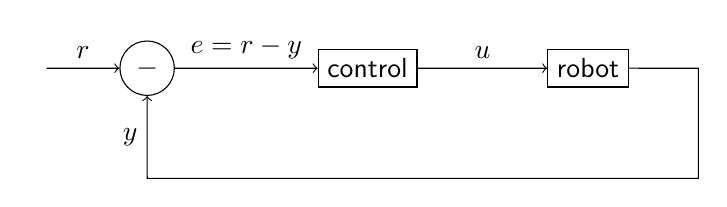
\begin{tikzpicture}[scale=1.4]
\node (input) at (0,1) {};
\node[circle,draw] (diff) at (1,1) {$-$};
\node[rectangle,draw] (control) at (3,1) {\textsf{control}};
\node[rectangle,draw] (robot) at (5,1) {\textsf{robot}};
\draw[->] (input) -- node[above] {$r$} (diff);
\draw[->] (diff)  -- node[above] {$e=r-y$} (control);
\draw[->] (control) -- node[above] {$u$} (robot);
\draw[->] (robot) -- ++(1,0) -- ++(0,-1) -- ++(-5,0) -- node[left] {$y$} (diff);
\end{tikzpicture}
\caption{A closed loop control system}\label{fig.control-model}
\end{center}
\end{figure}

The model in Fig.~\ref{fig.control-model} is also called a \emph{feedback control system} because the output value $y$ is fed back to the control algorithm and used to compute the control value. The output is compared with the reference value to compute $e=r-y$, the \emph{error}. The control algorithm uses the error to generate the control signal $u$ that is the input to the robot.

\subsection{The period of a control algorithm}
\index{control!algorithm!period of}

Control algorithms are run periodically (Algorithm~\ref{alg.control-loop}). The robot's software initializes a \emph{timer variable} to the required duration of the period to run the algorithm, for example, every $20$ ms. The embedded computer has a \emph{hardware clock} that ``ticks'' at fixed intervals causing an interrupt. The interrupt is handled by the operating system which decrements the value of the timer variable. When the value of this variable goes to zero, the timer has expired, and an event is raised in the software causing the control algorithm to be run.

\begin{figure}
\begin{alg}{Control algorithm outline}{control-loop}
\hline
&\idv{}integer period&// Duration of timer period\\
&\idv{}integer timer&// Timer variable\\
\hline
\stl{}&period \ass $\cdots$&// Period in milliseconds\\
\stl{}&timer \ass period&// Initialize the timer\\
\stl{}&loop&\\
\stl{}&\idc{}when timer-expired-event occurs&\\
\stl{}&\idc{}\idc{}control algorithm&// Run the algorithm\\
\stl{}&\idc{}\idc{}timer \ass period&// Reset the timer\\
\hline\hline
&// {\bfseries Operating system}&\\
\stl{}&when hardware-clock-interrupt occurs&\\
\stl{}&\idc{} timer \ass timer $-$ $1$&// Decrement the timer\\
\stl{}&\idc{} if timer $=$ $0$&// If the timer expires\\
\stl{}&\idc{}\idc{} raise timer-expired-event&// \ \ \ \ raise an event\\
\end{alg}
\end{figure}

The period of the algorithm is an important parameter in the design of a control system. If the period is too short, valuable computing resources will be wasted and the computer can become overloaded to the point that commands to the robot arrive too late. If the period is too long, the robot will not respond in time to correct errors in its motion.

\medskip

\noindent\textbf{Example} Consider a robot approaching an object that is $10$ cm away at $2$ cm/s. A control period of $1$ ms would waste computing resources because the robot will move only $0.002$ cm ($0.02$ mm) during \emph{each} $1$ ms cycle of the control algorithm. Changes in motor power over such small distances won't affect the ability of the robot to fulfill its task. At the opposite extreme, a control period of $2$ s is even worse: the robot will move $4$ cm during this period and will likely to crash into the object. A control period of roughly $0.25$ s ($250$ ms) during which the robot moves $0.5$ cm seems a reasonable value to start with since $0.5$ cm is a distance that is meaningful in terms of approaching an object. You can experiment with periods around this value to determine the optimum period: one that achieves satisfactory behavior with a period that is as long as possible to reduce the cost of computation.

\begin{framed}
\act{Setting the control period}{setperiod}
\begin{itemize}
\item In the example, we came to the conclusion that the optimum period of the control algorithm was of the order of magnitude of tenths of a second. In this activity we ask you consider what the optimum period should be for other control algorithms.
\item A home heating system contains a thermostat for controlling the temperature. What would be an optimum period for the control algorithm? The period depends on the engineering parameters of the heating system and on the physical properties of how the heat is transferred to the rooms. Explain how you would measure these factors and how they affect the control period.
\item Consider a self-driving car trying to park. What assumptions do you need to make to design a control period? What would be a reasonable period?
\item How do the properties of the sensors affect the control period? For the example of a robot approaching an object, how would the period change if the sensor can detect the object at $2$ cm, $5$ cm, $10$ cm, $20$ cm, $40$ cm?
\end{itemize}
\end{framed}

%\section{Control algorithms}\label{s.control-alg}
\index{control!algorithm}

We now define a sequence of four control algorithms, each one building on the previous one and providing more accurate control, at the price of more computational complexity. In practice, the system designer should choose the simplest algorithm that enables the robot to fulfill its task.

The algorithms are presented in the context of a robot which must approach an object and stop at a distance $s$ in front of it. The distance is measured by a proximity sensor and the speed of the robot is controlled by setting the power of the motors.


\section{On-off control}\label{s.on-off}
\index{control!algorithm!on-off}

The first control algorithm is called the \emph{on-off} or \emph{bang-bang} algorithm (Algorithm~\ref{alg.onoff}). We define a constant \p{reference} that is the distance in front of the object at which the robot is to stop. The variable \p{measured} is the actual distance measured by the proximity sensor. The \p{error} is the difference between the two:
\begin{center}
\p{error} $\leftarrow$ \p{reference} $-$ \p{measured},
\end{center}
which is negative if the robot is too far away from the object and positive if it is too close to the object. The motor powers are turned to full forwards or full backwards depending on the sign of the error. For example, if the reference distance is $10$ cm and the measured distance is $20$ cm, the robot is too far away and the error is $-10$ cm. Therefore, the motors must be set to move forwards.
\begin{figure}
\begin{alg}{On-off controller}{onoff}
&\idv{}integer reference \ass $\cdots$&// Reference distance\\
&\idv{}integer measured &// Measured distance\\
&\idv{}integer error &// Distance error\\
\hline
\stl{}&error \ass reference $-$ measured&\\
\stl{}&if error $<$ 0&\\
\stl{}&\idc{} left-motor-power \ass $100$&// Move forwards\\
\stl{}&\idc{} right-motor-power \ass $100$&\\
\stl{}&if error $=$ 0&\\
\stl{}&\idc{} left-motor-power \ass $0$&// Turn off motors\\
\stl{}&\idc{} right-motor-power \ass $0$&\\
\stl{}&if error $>$ 0&\\
\stl{}&\idc{} left-motor-power \ass $-100$&// Move backwards\\
\stl{}&\idc{} right-motor-power \ass $-100$&\\
\end{alg}
\end{figure}

The robot approaches the object at full speed. When the robot reaches the reference distance from the object, it takes time for the sensor to be read and the error to be computed. Even if the robot measures a distance exactly equal to the reference distance (which is unlikely), the robot will not be able to stop immediately and will overrun the reference distance. The algorithm will then cause the robot to back up at full speed, again passing the reference distance. When the timer causes the control algorithm to be run again, the robot will reverse direction and go forwards at full speed. The resulting behavior of the robot is shown in Fig.~\ref{fig.onoff}: the robot will oscillate around the reference distance to the object. It is highly unlikely that the robot will actually stop at or near the reference distance.

\begin{figure}
\begin{center}
\begin{tikzpicture}[scale=1.2]
\draw[<->] (0,5) -- node[sloped,above,rotate=180] {\p{distance}} (0,0) node[left] {} -- node[below] {\p{time}} (8,0);
\draw (0,2) node[below right] {$r$} -- (8,2);
\draw[thick] plot coordinates {(0,5) (2,1.5) (3,2.5) (4,1.5) (5,2.5) (6,1.5)(7,2.5) (8,1.5)};
\end{tikzpicture}
\caption{Behavior of the on-off algorithm}\label{fig.onoff}
\end{center}
\end{figure}

A further disadvantage of the on-off algorithm is that the frequent and abrupt reversal of direction results in high accelerations. If we are trying to control a gripper arm, the objects that it is carrying may be damaged. The algorithm generates high levels of wear and tear on the motors and on other mechanical moving parts.

\begin{framed}
\act{On-off controller}{onoff}
\begin{itemize}
\item Implement the on-off algorithm on your robot for the task of stopping at a reference distance from an object.
\item Run it several times starting at differences distances from the object.
\item Algorithm~\ref{alg.onoff} stops the robot when the error is exactly zero. Modify the implementation so that the robot stops if the error is within a small range around zero. Experiment with different ranges and see how they affect the behavior of the robot.
\end{itemize}
\end{framed}

\section{Proportional (P) controller}\label{s.p}
\index{control!algorithm!proportional}

To develop a better algorithm, we take inspiration from riding a bicycle. Suppose that you are riding your bicycle and see that the traffic light ahead has turned red. You don't wait until the last moment when you are at the stop line and then squeeze hard on the brake lever; if you do so, you might be thrown from the bicycle! What you do is to slow your speed gradually: first, you stop pedaling; then, you squeeze the brake gently to slow down a bit more; finally, when you are at the stop line and going slowly, you squeeze harder to fully stop the bicycle. The algorithm used by a bicycle rider can be expressed as:
\begin{quote}
\normalsize\noindent{}Reduce your speed more as you get closer to the reference distance.
\end{quote}
The decrease in speed is (inversely) \emph{proportional} to how close you are to the traffic light: the closer you are, the more you slow down. The factor of proportionality is called the \emph{gain}\index{control!algorithm!gain} of the control algorithm. An alternate way of expressing this algorithm is:
\begin{quote}
\normalsize\noindent{}Reduce your speed more as the error between the reference distance and the measured distance gets smaller.
\end{quote}

Algorithm~\ref{alg.proportional} is the \emph{proportional control algorithm} or a \emph{P-controller}.

\begin{figure}
\begin{alg}{Proportional controller}{proportional}
&\idv{}integer reference \ass $\cdots$&// Reference distance\\
&\idv{}integer measured &// Measured distance\\
&\idv{}integer error &// Error\\
&\idv{}float gain \ass $\cdots$& // Proportional gain\\
&\idv{}integer power & // Motor power\\
\hline
\stl{}&error \ass reference $-$ measured&// Distances\\
\stl{}&power \ass gain * error&// Control value\\
\stl{}&left-motor-power \ass power&\\
\stl{}&right-motor-power \ass power&\\
\end{alg}
\end{figure}

\medskip

\noindent\textbf{Example} Suppose that the reference distance is $100$ cm and the gain is $-0.8$. When the robot is $150$ cm away from the object, the error is $100-150=-50$ and the control algorithm will set the power to $-0.8\cdot -50=40$. Table~\ref{tab.p-controller} shows the errors and power settings for three distances. If the robot overruns the reference distance of $100$ cm and a distance of $60$ cm is measured, the power will be set to $-32$ causing the robot to move backwards.

\begin{table}
\caption{Proportional controller for gain of $-0.8$}
\label{tab.p-controller}
\begin{tabular}{rrr}
\svhline\noalign{\smallskip}
\multicolumn{1}{c}{distance} & \multicolumn{1}{c}{\ \ \ error}& \multicolumn{1}{c}{\ \ \ power}\\
\noalign{\smallskip}\svhline\noalign{\smallskip}
$150$ & $-50$ & $40$\\
$125$ & $-25$ & $20$\\
$60$ & $40$ & $-32$\\
\noalign{\smallskip}\svhline\noalign{\smallskip}
\end{tabular}
\end{table}

Figure~\ref{fig.p-control} plots the distance of the robot to the object as a function of time when the robot is controlled by a P controller. The line labeled $r$ is the reference distance. The change in the motor power is smooth so the robot doesn't experience rapid accelerations and decelerations. The response is somewhat slow, but the robot does approach the target distance.

\begin{figure}
\begin{center}
\begin{tikzpicture}[scale=1.2]
\draw[<->] (0,5) -- node[sloped,above,rotate=180] {\p{distance}} (0,0) node[left] {} -- node[below] {\p{time}} (8,0);
\draw (0,1.9) node[below right] {$r$} -- (8,1.9);
\draw[domain=0:8,samples=100,thick] plot (\x,{3*exp(-2*\x)+2});
\end{tikzpicture}
\caption{Behavior of the P controller}\label{fig.p-control}
\end{center}
\end{figure}

Unfortunately, the robot does not actually reach the reference distance. To understand why this happens, consider what happens when the robot is very close to the reference distance. The error will be very small and consequently the power setting will be very low. In theory, the low power setting should cause the robot to move slowly, eventually reaching the reference distance. In practice, the motor power may become so low that it is not able to overcome the internal friction in the motors and their connection to the wheels, so the robot stops moving.

It might seem that increasing the gain of the P controller could overcome this problem, but a high gain suffers from a serious disadvantage. Figure~\ref{fig.gain} shows the effect of the gain on the P controller. Higher gain (dashed red line) causes the robot to approach the reference distance faster, while lower gain (dotted blue line) causes the robot to approach the reference distance slower. However, if the gain is too high, the P controller functions like an on-off controller with an oscillating response (green line). We say that the controller is \emph{unstable}.

\begin{figure}
\begin{center}
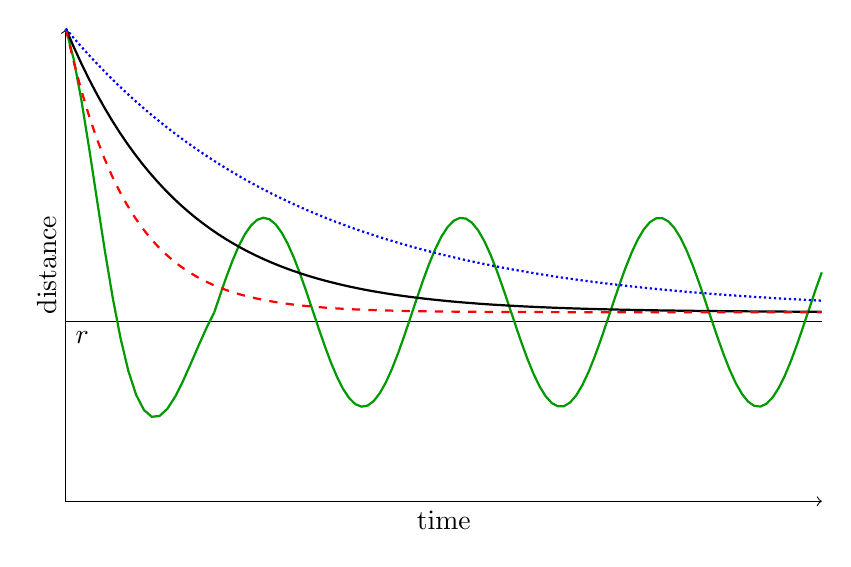
\begin{tikzpicture}[scale=1.2]
\draw[<->] (0,5) -- node[sloped,above,rotate=180] {\p{distance}} (0,0) node[left] {} -- node[below] {\p{time}} (8,0);
\draw (0,1.9) node[below right] {$r$} -- (8,1.9);
\draw[domain=0:1.57,samples=20,thick,green!60!black] plot (\x,{3*exp(-\x)*cos(3*\x r)+2});
\draw[domain=1.57:8,samples=100,thick,green!60!black] plot (\x,{cos(3*\x r)+2});
\draw[domain=0:8,samples=100,thick] plot (\x,{3*exp(-.8*\x)+2});
\draw[domain=0:8,samples=100,dashed,red,thick] plot (\x,{3*exp(-1.5*\x)+2});
\draw[domain=0:8,samples=100,densely dotted,blue,thick] plot (\x,{3*exp(-.4*\x)+2});
\end{tikzpicture}
\caption{The effect of the gain on the P controller: lower gain (dotted blue line), higher gain (dashed red line), excessive gain (oscillating green line)}\label{fig.gain}
\end{center}
\end{figure}

There are situations where the P controller cannot reach the reference distance even in a ideal system. Suppose that the object itself is moving at constant speed away from the robot. The P controller will set maximum motor power to cause the robot to move rapidly towards the object. Eventually, however, as the robot approaches the object, the measured distance will become small and the P controller will set the power so low that the speed of the robot is lower than the speed of the object. The result is that the robot will never reach the reference distance. If the robot could actually reach the reference distance, the error would be zero and therefore the speed of the robot would also be zero. The object, however, is still moving away from the robot, so somewhat later the robot will start moving again and the cycle repeats. This start-and-stop motion is not the intended goal of maintaining the reference distance.

\smallskip

\noindent\textbf{Example} We use the same data as in the previous example except that the object moves at $20$ cm/s. Table~\ref{tab.p-controller-moving} shows the errors and power settings for three distances. Initially, the robot is going faster then the object so it will catch up. At $125$ cm from the object, however, the robot is moving at the same speed as the object. It maintains this fixed distance and will not approach the reference distance of $100$ cm. If somehow the robot gets closer to the object, say, $110$ cm,  the power is reduced to $8$ causing the robot to back away from the object.

\begin{table}
\caption{Proportional controller for a moving object and a gain of $-0.8$}
\label{tab.p-controller-moving}
\begin{tabular}{rrr}
\svhline\noalign{\smallskip}
\multicolumn{1}{c}{distance} & \multicolumn{1}{c}{\ \ \ error}& \multicolumn{1}{c}{\ \ \ power}\\
\noalign{\smallskip}\svhline\noalign{\smallskip}
$150$ & $-50$ & $40$\\
$125$ & $-25$ & $20$\\
$110$ & $-10$ & $8$\\
\noalign{\smallskip}\svhline\noalign{\smallskip}
\end{tabular}
\end{table}

In general, the robot will stabilize at a fixed distance from the reference distance. You can reduce this error by increasing the gain, but the reference distance will never be reached and the only result is that the controller becomes unstable.

\begin{framed}
\act{Proportional controller}{proportional}
\begin{itemize}
\item Implement the proportional control algorithm to cause the robot to stop at a specified distance from an object. How accurately can you achieve the goal when the object does not move?
\item What happens if the object moves? For the object you can use a second robot programmed to move at a fixed speed.
\item Experiment with the gain and the period to see how they affect the performance of the algorithm.
\end{itemize}
\end{framed}

\section{Proportional-integral (PI) controller}\label{s.pi}
\index{control!algorithm!proportional-integral}

A \emph{proportional-integral controller} can achieve the reference distance even in the presence of friction or a moving object by taking into account the accumulated error over time. Whereas the P controller only takes into account the current error:
\[
u(t) = k_pe(t)\,,
\]
the PI controller adds the integral of the error from the time when the algorithm starts to run until the present time:
\[
u(t) = k_pe(t) + k_i\int_{0}^t e(\tau)\,d\tau\,.
\]
Separate gain factors are used for the proportional and integral terms to allow flexibility in the design of the controller.

When implementing a PI controller, a discrete approximation to the continuous integral is performed (Algorithm~\ref{alg.pi-controller}).

\begin{figure}
\begin{alg}{Proportional-integral controller}{pi-controller}
&\idv{}integer reference \ass $\cdots$&// Reference distance\\
&\idv{}integer measured &// Measured distance\\
&\idv{}integer error &// Error\\
&\idv{}integer error-sum $\leftarrow 0$&// Cumulative error\\
&\idv{}float gain-p \ass $\cdots$& // Proportional gain\\
&\idv{}float gain-i \ass $\cdots$& // Integral gain\\
&\idv{}integer power & // Motor power\\
\hline
\stl{}&error \ass reference $-$ measured&// Distances\\
\stl{}&error-sum \ass error-sum + error&// Integral term\\
\stl{}&power \ass gain-p * error + gain-i * error-sum&// Control value\\ 
\stl{}&left-motor-power \ass power&\\
\stl{}&right-motor-power \ass power&\\
\end{alg}
\end{figure}

In the presence of friction or a moving object, the error will be integrated and cause a higher motor power to be set; this will cause the robot to converge to the reference distance. A problem with a PI controller is that the integration of the error starts from the initial state when robot is far from the object. As the robot approaches the reference distance, the integral term of the controller will have already a large value; to decrease this value the robot must move past the reference distance so that there are errors of opposite sign. This can generate oscillations (Fig.~\ref{fig.pi-control}).

\begin{figure}
\begin{center}
\begin{tikzpicture}[scale=1.2]
\draw[<->] (0,5) -- node[sloped,above,rotate=180] {\p{distance}} (0,0) node[left] {} -- node[below] {\p{time}} (8,0);
\draw (0,2) node[below right,xshift=-1pt] {$r$} -- (8,2);
\draw[domain=0:8,samples=100,thick] plot (\x,{3*exp(-1*\x)*cos(5*\x r)+2});
\end{tikzpicture}
\caption{Behavior of the PI controller}\label{fig.pi-control}
\end{center}
\end{figure}

\begin{framed}
\act{PI controller}{PIcontroller}
\begin{itemize}
\item Implement a PI controller that causes the robot to stop at a specified distance from an object.
\item Compare the behavior of the PI controller with a P controller for the same task by monitoring the variables of the control algorithms over time.
\item What happens if you manually prevent the robot from moving for a short time and then let it go? This demonstrates a concept called \emph{integrator windup}\index{control!integrator windup}. Explore the concept through online sources and find a method to fix the problem.
\end{itemize}
\end{framed}

\section{Proportional-integral-derivative (PID) controller}\label{s.pid}
\index{control!algorithm!proportional-integral-derivative}

When you throw or kick a ball to another player who is moving, you do not throw it to his current position. By the time the ball reaches him, he will have moved to a new position. Instead, you estimate where the new position will be and aim the ball there. Similarly, a robot whose task is to push a parcel onto a moving trolley must time its push to the estimated future position of the trolley when the parcel reaches it. The control algorithm of this robot cannot be an on-off, P or PI controller, because they only take into account the current value of the error (and for the PI controller the previous values). 

To estimate the future error, the rate of change of the error can be taken into account. If the rate of change of the error is small, the robot can push the parcel just before the trolley approaches it, while if the rate of change of the error is large, the parcel should be pushed much earlier.

Mathematically, rate of change is expressed as a derivative. A \emph{proportional-integral-derivative (PID)} controller adds an additional term to P and I terms:
\begin{equation}
u(t) = k_pe(t) + k_i\int_{\tau=0}^t e(\tau)\,d\tau + k_d \frac{de(t)}{dt}\,.\label{eq.pid}
\end{equation}

In the implementation of a PID controller, the differential is approximated by the difference between the previous error and current error (Algorithm~\ref{alg.pid-controller}).

\begin{figure}
\begin{alg}{Proportional-integral-differential controller}{pid-controller}
&\idv{}integer reference \ass $\cdots$&// Reference distance\\
&\idv{}integer measured &// Measured distance\\
&\idv{}integer error &// Error\\
&\idv{}integer error-sum $\leftarrow 0$ &// Cumulative error\\
&\idv{}integer previous-error \ass 0&// Previous error\\
&\idv{}integer error-diff &// Error difference\\
&\idv{}float gain-p \ass $\cdots$& // Proportional gain\\
&\idv{}float gain-i \ass $\cdots$& // Integral gain\\
&\idv{}float gain-d \ass $\cdots$& // Derivative gain\\
&\idv{}integer power & // Motor power\\
\hline
\stl{}&error \ass reference $-$ measured&// Distances\\
\stl{}&error-sum \ass error-sum + error&// Integral term\\
\stl{}&error-diff \ass error $-$ previous-error&// Differential term\\
\stl{}&previous-error \ass error&// Save current error\\
\stl{}&power \ass gain-p * error + &// Control value\\ 
&\idc{}gain-i * error-sum + gain-d * error-diff&\\ 
\stl{}&left-motor-power \ass power&\\
\stl{}&right-motor-power \ass power&\\
\end{alg}
\end{figure}

The behavior of the PID controller is shown in Fig.~\ref{fig.pid-control}. The robot smoothly and rapidly converges to the reference distance. 

\begin{figure}
\begin{center}
\begin{tikzpicture}[scale=1.2]
\draw[<->] (0,5) -- node[sloped,above,rotate=180] {\p{distance}} (0,0) node[left] {} -- node[below] {\p{time}} (8,0);
\draw[dashed] (0,2) node[below right] {$r$} -- (8,2);
\draw[domain=0:8,samples=100,thick] plot (\x,{2.5*exp(-2*\x)+2});
\end{tikzpicture}
\caption{Behavior of the PID controller}\label{fig.pid-control}
\end{center}
\end{figure}

The gains of a PID controller must be carefully balanced. If the gains for the P and I terms are too high, oscillations can occur. If the gain for the D term is too high, the controller will react to short bursts of noise.


\begin{framed}
\act{PID controller}{PIDcontroller}
\begin{itemize}
\item Implement a PID controller for the task of a robot approaching an object.
\item Experiment with different gains until the robot smoothly approaches the reference distance.
\item Repeat the experiments with a moving object.
\end{itemize}
\end{framed}

\section{Summary}

A good control algorithm should converge rapidly to the desired result while
avoiding abrupt motion. It must be computationally efficient, but not require constant tuning. The control algorithm has to be adapted to the specific requirements of the system and the task, and to function correctly in different environmental conditions. We have described four algorithms, from the impractical on-off algorithm through algorithms that combine proportional, integral and derivative terms. The proportional term ensures that large errors cause rapid convergence to the reference, the integral term ensures that the reference can actually be attained, while the derivative term makes the algorithm more responsive. 

\section{Further reading}

A modern textbook on control algorithms is \cite{astrom-murray}.

\bibliographystyle{spmpsci}
\bibliography{er}
